
%% bare_conf.tex
%% V1.4b
%% 2015/08/26
%% by Michael Shell
%% See:
%% http://www.michaelshell.org/
%% for current contact information.
%%
%% This is a skeleton file demonstrating the use of IEEEtran.cls
%% (requires IEEEtran.cls version 1.8b or later) with an IEEE
%% conference paper.
%%
%% Support sites:
%% http://www.michaelshell.org/tex/ieeetran/
%% http://www.ctan.org/pkg/ieeetran
%% and
%% http://www.ieee.org/

%%*************************************************************************
%% Legal Notice:
%% This code is offered as-is without any warranty either expressed or
%% implied; without even the implied warranty of MERCHANTABILITY or
%% FITNESS FOR A PARTICULAR PURPOSE!
%% User assumes all risk.
%% In no event shall the IEEE or any contributor to this code be liable for
%% any damages or losses, including, but not limited to, incidental,
%% consequential, or any other damages, resulting from the use or misuse
%% of any information contained here.
%%
%% All comments are the opinions of their respective authors and are not
%% necessarily endorsed by the IEEE.
%%
%% This work is distributed under the LaTeX Project Public License (LPPL)
%% ( http://www.latex-project.org/ ) version 1.3, and may be freely used,
%% distributed and modified. A copy of the LPPL, version 1.3, is included
%% in the base LaTeX documentation of all distributions of LaTeX released
%% 2003/12/01 or later.
%% Retain all contribution notices and credits.
%% ** Modified files should be clearly indicated as such, including  **
%% ** renaming them and changing author support contact information. **
%%*************************************************************************


% *** Authors should verify (and, if needed, correct) their LaTeX system  ***
% *** with the testflow diagnostic prior to trusting their LaTeX platform ***
% *** with production work. The IEEE's font choices and paper sizes can   ***
% *** trigger bugs that do not appear when using other class files.       ***
%                       ***
% The testflow support page is at:
% http://www.michaelshell.org/tex/testflow/



\documentclass[conference]{IEEEtran}


% *** CITATION PACKAGES ***
%
%\usepackage{cite}
% cite.sty was written by Donald Arseneau
% V1.6 and later of IEEEtran pre-defines the format of the cite.sty package
% \cite{} output to follow that of the IEEE. Loading the cite package will
% result in citation numbers being automatically sorted and properly
% "compressed/ranged". e.g., [1], [9], [2], [7], [5], [6] without using
% cite.sty will become [1], [2], [5]--[7], [9] using cite.sty. cite.sty's
% \cite will automatically add leading space, if needed. Use cite.sty's
% noadjust option (cite.sty V3.8 and later) if you want to turn this off
% such as if a citation ever needs to be enclosed in parenthesis.
% cite.sty is already installed on most LaTeX systems. Be sure and use
% version 5.0 (2009-03-20) and later if using hyperref.sty.
% The latest version can be obtained at:
% http://www.ctan.org/pkg/cite
% The documentation is contained in the cite.sty file itself.


% *** GRAPHICS RELATED PACKAGES ***
%
\ifCLASSINFOpdf \usepackage[pdftex]{graphicx} \usepackage{wrapfig} % declare the
% path(s) where your graphic files are
\graphicspath{{pic/}} % and their extensions so you won't have to specify these
% with
% every instance of \includegraphics
\DeclareGraphicsExtensions{.png} \else % or other class option (dvipsone,
% dvipdf, if not using dvips). graphicx
% will default to the driver specified in the system graphics.cfg if no
% driver is specified.
% \usepackage[dvips]{graphicx}
% declare the path(s) where your graphic files are
% \graphicspath{{../eps/}}
% and their extensions so you won't have to specify these with
% every instance of \includegraphics
% \DeclareGraphicsExtensions{.eps}
\fi

% correct bad hyphenation here
\hyphenation{op-tical net-works semi-conduc-tor}


\begin{document} \title{A Tool for Visualizing Patterns of Spreadsheet Function
		Combinations}
	
	
	% author names and affiliations
	% use a multiple column layout for up to three different
	% affiliations
	\author{\IEEEauthorblockN{Justin A. Middleton} \IEEEauthorblockA{North Carolina
			State University\\ Raleigh, North Carolina}}
	
	
	% use for special paper notices
	%\IEEEspecialpapernotice{(Invited Paper)}
	
	
	
	
	% make the title area
	\maketitle
	
	% As a general rule, do not put math, special symbols or citations
	% in the abstract
	\begin{abstract} Spreadsheet environments often come equipped with an abundance
		of functions and operations to manipulate data, but it can be difficult to
		understand how programmers actually use these in practice. Furthermore, users
		can combine several functions into a complex formula, complicating matters for
		both researchers and practitioners who want to study formulae to improve
		spreadsheet practices. Therefore, we developed a tool that visualizes patterns
		of function combination in spreadsheets as an interactive tree of
		possibilities. Using spreadsheets from the public spreadsheet corpora, we then
		apply to the tool to real datasets and demonstrate its ability to capture the
		most common and most anomalous patterns of function combination and their
		contexts in actual workbooks. \end{abstract}
	
	\section{Introduction} Business and research alike a lot to spreadsheets, the
	tabular interface that offers users a structured way to store and manipulate
	potentially huge bodies of data. Their allure is in their versatility: while
	the novice can still work without a deep knowledge of programming, they can
	learn to expedite their work by building programs out of several available
	functions \cite{nardi1990spreadsheet}. As such, it should not be surprising
	that when Scaffidi and colleagues estimated that over 50 million U.S. workers
	could be using them by 2012, with 25 million of them writing programs 
	\cite{scaffidi2005estimating}. \par Considering this ubiquity, it's crucial to
	understand how people are actually using spreadsheets. After all, failures in
	their practice can be ruinous, as demonstrated in EuSpRIG's many horror stories
	of spreadsheets gone wrong. In 2013, for example, they detail the influence of
	an economics paper on debt and national growth which shaped many political
	initiates around it, only to discover that the spreadsheets used in the data
	analysis contained an error that reversed the findings. The other stories,
	likewise, do not augur well if shoddy spreadsheet practices persist
	\footnote{http://www.eusprig.org/horror-stories.htm}. \par Fortunately, many
	spreadsheet researchers have assembled and released a number of spreadsheet
	corpora to inform work of how people actually use these tools. Collections like
	EUSES \cite{fisher2005euses}, FUSE \cite{barik2015fuse}, and the Enron corpus
	\cite{hermans2015enron} have already enabled fruitful work across the field.
	Hermans and colleagues, for example, used the EUSES corpus in 2011 to inform
	and evaluate their work on exploring code smells, or inelegant places in code
	that suggest the need for refactoring, between worksheets
	\cite{hermans2012detecting}. \par A tool, then, that empowers users of any
	intention to explore these datasets would be rife with potential. On a simple
	level, the tool could provide concrete statistics on which functions are used
	in practice most (or least) often for a given dataset. Beyond this, though, it
	could also inform future work on recommending functions through an
	understanding of this patterns, or it could guide API improvement by suggesting
	functions to add or prune based how people actually use them. Furthermore, if
	the tool maintains the connection between its broad patterns and the actual
	instances of formulae in workbooks, it could serve as a boon to educators not
	only by showing which functions and combinations are most practical to learn
	but also by offering a bounty of instructive, and real, examples \par This
	paper contributes a tool, informed by some of the aforementioned spreadsheet
	corpora, that seeks to accomplish these tasks by offering an interactive
	interface for exploring how people combine functions. It seeks to balance
	several needs, such as capturing these patterns in a broad enough overview
	while still be specific enough lead back to the precise places in spreadsheets
	where these patterns are realized. Along with the tool, then, is also a
	discussion of the various goals which the tool seeks to fulfill and the
	trade-offs that we negotiated at each point. All of this culminates in an
	evaluation of the tool through a study of possible cases to which the tool
	might apply.
	
	\section{Related Work} This tool comes from a line of spreadsheet visualization
	tools before it, each with a different focus. Some tools, such as Igarashi and
	colleague's fluid visualizations \cite{igarashi1998fluid}, seek to visualize
	the hidden formulas within a spreadsheet by imposing the dataflow graphs over
	the cells. Likewise, Clermont \cite{clermont2003scalable} (and Hipfl
	\cite{hipfl2008using}, who extended his work) explored various ways of
	visualizing groups of related cells through similar functions, neighbors, or
	references. Others focus on creating visualizations outside of the sheets:
	Hermans and colleagues address a spreadsheet programmer's information needs
	through their work on the tools GyroSAT \cite{hermans2011supporting} and Breviz
	\cite{hermans2011breviz} to make dataflow diagrams of individual spreadsheets.
	These, however, tend to focus on individual spreadsheets and not bodies of
	them. \par Nevertheless, other studies and tools focus more on evaluating the
	content of the cells therein. Badame, for example, implements a number of Excel
	formula refactorings and uses Euses in part to evaluate it
	\cite{badame2012refactoring}. Hermans, leveraging her work with the
	aforementioned dataflow diagrams, approached the same dataset to assess the
	prevalence of common inter-worksheet smells, such as feature envy and
	inappropriate intimacy \cite{hermans2012detecting}. Cunha and colleagues,
	likewise, constructed and refined a catalogue of smells and implemented the
	SmellSheet Detective tool to detect bad smells in chosen spreadsheets
	\cite{cunha2012towards}, which Abreu and colleagues later extended to detect
	faults. \cite{abreu2014smelling}.\par Implicit in this study is an exploration
	of how users interact with the Excel API. Previous research, such as the first
	study on the Enron spreadsheet corpus \cite{hermans2015enron}, on how users
	employ certain functions or commands. Researchers have applied such questions
	to other contexts as well, such as Murphy and colleague's study into how Java
	developers use Eclipse and what commands they use most often
	\cite{murphy2006java}.  Others focus on the documentation of the API itself:
	Robillard and DeLine, for example conducted a series of surveys and interviews
	to diagnose common problems with learning APIs, and they found that code
	examples, one of the focuses of this tool, is one of the most important aids to
	have in learning a new system \cite{robillard2011field}.
	
	\section{Approach/Methodology} \subsection{Walkthrough of Tool} Before
	discussing the minutiae of how the tool was developed, it will help first to
	give a basic example of how the tool can be used and how to interpret its
	symbols. One such example might be to find the answer to this question:
	\textit{ What kinds of functions do people use to define the condition in an IF
		function?} The final visualization is available in figure \ref{fig:fullpic};
	however, to understand the interaction, we will start rather from the
	beginning. \par When the user first approaches the tree for a given top-level
	function -- that is, a function nested within none other -- only a few nodes
	are visible, as shown in figure \ref{fig:startpic}. \par
	
	\centerline{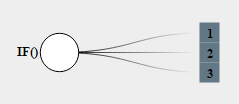
\includegraphics{start}}
	
	The visualization so far comprises two types of node: the circle, which
	represents a discrete function in the formula and is size according to its
	relative frequency (the top-level node, by definition, will be the largest);
	and the numbered squares, which represent the positions of arguments within its
	parent function. From this, we can infer that, of the times it was observed, IF
	can have at most three arguments passed into it, which corresponds with its
	specifications in the
	API.\footnote{https://support.office.com/en-us/article/IF-function-69aed7c9-4e8a-4755-a9bc-aa8bbff73be2} \par Knowing that it is the first argument which contains the conditionals, we click on the square labeled "1" to explore. To save space, when more than 10 unique arguments have been observed in any position, the tool displays only the first ten, with an option to display the rest. The results are shown below:
	
	\centerline{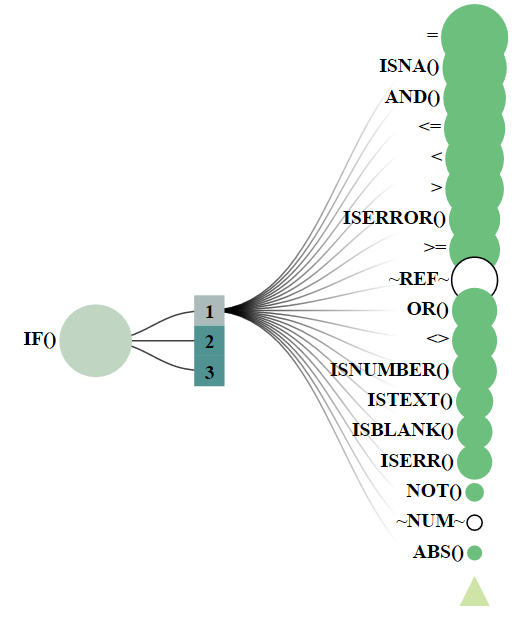
\includegraphics[width=.43\textwidth]{IFexpand}}
	
	As expected, we see that IF contains as its first argument a number of
	comparison operators, such as = and <=, and boolean-returning functions, like
	ISNA and AND, with simple equality being the most common and some use as ABS
	being the least seen of everything actually used. \par From here, we can
	further explore the common options among these functions. Clicking on the "="
	node will yield two arguments, it being a binary operator, and expanding each
	of them will peer into the range of common values of equality comparison, which
	Figure \ref{fig:fullpic} shows. \par For both sides of the equal sign, the
	operator has certain types of arguments which predominate over the others: on
	the left side is most often a reference to another cell; on the right, a string
	or number literal, which makes sense for the case of confirming a value in
	another cell before assigning this one. Furthermore, if the concept is
	difficult to imagine is practice, a tooltip accompanies each function node in
	the tree, providing a concrete example of a function that uses this structure
	and where it can be found. If this single instance is not enough, then the user
	also has the option to double-click the individual function node, which will
	open up a new tab with a table of many more examples from dataset.
	
	\begin{figure*}[t] 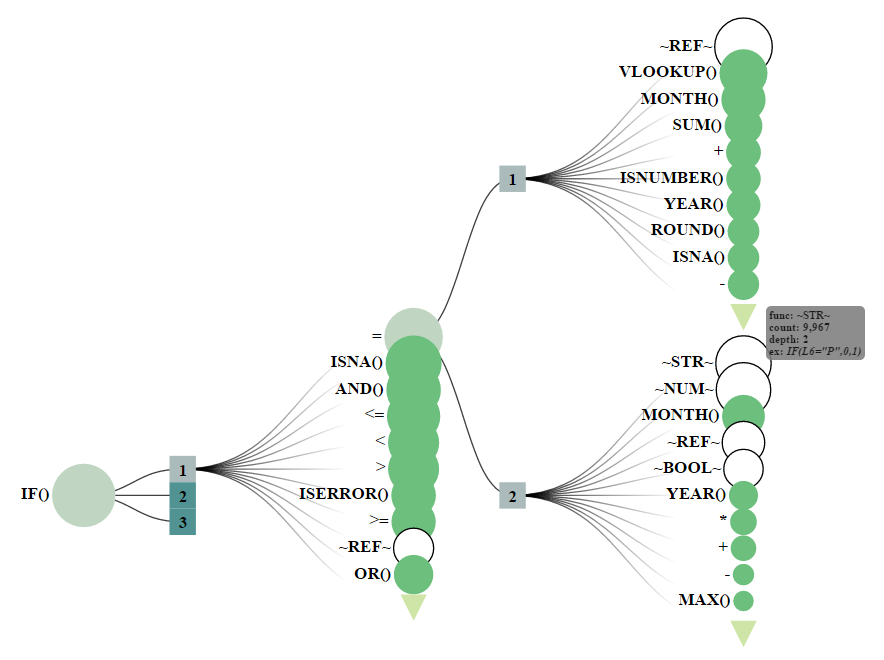
\includegraphics[width = \textwidth]{IFargslabel} \caption{A
			picture of the tool.} \centering \label{fig:fullpic} \end{figure*}
	
	\subsection{Design Goals} In visualizing the spreadsheet data, I outlined a few
	core goals for what the tool should accomplish: \begin{itemize} \item [1]
		\textbf{Draw an interactive interface to explore observed function
			combinations.} The combination space for all Excel functions is massive, let
		alone the space for observed formulas. Working from data with actual referents
		in practice, the tool must aid the user in navigating this space. \item [2]
		\textbf{Emphasize the quantitative patterns in formula construction.} The tool,
		accommodating datasets of a few spreadsheets to millions, should address the
		questions of how often the end users employed a certain function and where they
		used it. In this way, it must show precise metrics, such as frequency of  use
		and depth of function nesting, of the dataset it conveys. \item [3]
		\textbf{Promote a qualitative understanding of the patterns.} Lest these
		patterns remain abstract, the tool should supplement its observations with
		concrete instances of relevant formulas from the corpus. Ideally, it should
		even direct users to the exact cell in the spreadsheets where the formula was
		used, contextualizing the functions. \end{itemize} \par Likewise, to bound our
	scope, we outlined a few goals to specifically avoid accomplishing with this:
	\begin{itemize} \item [!1] \textbf{Do not try to directly explain what a
			function does.} Though the tool tries to foster tries understanding by linking
		pattern to example, it won't provide a precise description of what a function
		accomplishes. The tool's user must infer this. \item [!2] \textbf{Do not create
			new formulas.} This is essentially an exploratory tool, not a generative one.
		It should not produce any information other than new views of the original
		data. \item [!3] \textbf{Do not visualize individual formulas.} Though there is
		room to explore the place of a single function in the group, the tool must
		design the core visualization around the entire body of data, not the other way
		around. \end{itemize}
	
	\subsection{Design Decisions} Early in the process, we decided that the tree
	form would be a suitable fit to represent the parent-child or caller-callee
	relationships inherent in the data, given the composition of formulas as
	functions and their arguments (which could be yet more functions). By adapting
	this structure to accommodate a broad range of possibilities for nested
	functions, the branching factor depends on both the number of arguments in a
	function and the number of possible functions observed as an argument in a
	function. \par Guided by the goals in section A, we faced a number of decision
	points, a sample of which we describe below, before we arrived at the design
	shown above. \begin{itemize} \item \textit{Copied formulas}: Excel allows users
		to spread a formula over an area, repeating the same task in each cell with
		minor adjustments. Without checking for this, the analysis may not reveal the
		functions most commonly used together but rather the formulas most often
		applied to large areas. To combat this, we converted formulas from their native
		A1 format to the relative R1C1, in which copied formulas should be identical,
		and reduced the records to unique R1C1 formulas per sheet. \item
		\textit{Importance of depth}: When a function appears within another, should it
		be analyzed only as a nested function or would it also be valid to analyze the
		nested function on its own?  \par For example, in the pictured IF function, we
		found that people often use another IF statement as the second or third
		arguments of the top-level IF. If we only consider functions exactly where
		they're found embedded in the formula, then information about the same function
		-- IF, in this case -- will be scattered across different trees with no way to
		aggregate them. If we record every instance of a function by ignoring their
		context -- that is, including an IF embedded within a SUM function in the same
		node as the top-level IF -- then the tool will represent some functions in
		multiple nodes to capture every possible level of nesting. Both approaches have
		benefits and drawbacks, and so we included both. \item \textit{Pattern
			density}: How should the tool quantitatively order its elements: by a
		function's raw frequency or by the unity of patterns it leads to? For example,
		if SUM has for its first argument two possibilities, one which itself contains
		1000 unique argument possibilities with 1 occurrence each (high frequency, low
		pattern density) and another seen with 2 argument possibilities of 100
		occurrences each (low frequency, high pattern density), which would be more
		interesting to emphasize? The answer depends on the nuances of the questions,
		but for simplicity, I've shown the former. \item \textit{Non-functions}: How
		should the tool represent everything in the formula that isn't a function:
		numbers, string literals, errors, references, etc? Since these don't accept
		arguments, they will adorn the tree as leaves, and their precise content won't
		affect the functions around them as long as their types are known. As such, in
		the visualization, all of these nodes are replaced and aggregated under their
		types and represented as empty white nodes. \item \textit{Optional arguments}:
		How should the tool handle functions which accept a variable number of
		arguments? SUM, for example, can have anywhere from 1 to 255, and IF can accept
		either 2 or 3.
		\footnote{https://support.office.com/en-us/article/Excel-functions-by-category-5f91f4e9-7b42-46d2-9bd1-63f26a86c0eb} Without prior evidence, it's possible that, when people use optional arguments, they use different kinds of types and functions for arguments versus the cases when they ignore optional arguments. To account for this, we separate and analyze the different quantities of arguments observed for each function; the tool, however, uses as default all of the options collapsed into a single representation. \end{itemize}
	
	\subsection{Implementation Details} We can view the final visualization as the
	product of two discrete processes: \begin{itemize} \item \textit{Collection}:
		Given a set of Excel sheets, the tool, written mostly in Java, uses Apache
		POI\footnote{https://poi.apache.org/} to identify and iterate over every cell
		containing a valid formula. Afterward, it calls POI's formula parser to break
		the formula text into an ordered set of individual tokens, which the tool then
		parses into the tree-like form by which it is recorded. When all formulas have
		been analyzed like this, it produces JSON files for each top-level function in
		the set. \item \textit{Presentation}: The JSON files, meanwhile, feed into the
		presentation code, implemented in Javascript with much help from the
		visualization library D3\footnote{https://d3js.org/}. We chose D3 primarily for
		its accessibility: given the JSON, the visualization can be rather simply
		embedded into a webpage accessible through a browser. \end{itemize} A
	demonstration of the tool can be found at [LINK HERE].
	
	\section{Case Study} The obvious question to pose to any visualization is this:
	Why does it matter that we see this way? In other words, it is not enough to
	prove that something can be visualized; instead we must also demonstrate what
	we can be gained from any particular visualization. As such, we raised a few
	tasks in the introduction in which we thought the tool could help: identifying
	places for API improvement, detecting bad smells or common programmer
	misunderstanding, and guiding spreadsheet education. To demonstrate the tool's
	applicability, then, we sought out places in the tree which best exemplify
	these respective concerns.
	
	\subsection{Bad Smells} Fowler's (?) seminal description of code smells
	underscored an important point of code quality: between perfect code and
	bug-crippled spaghetti,  there is a spectrum of code designs which, by
	themselves, are not faulty but nevertheless suggest problems and
	vulnerabilities in code design. Code smells, as we call them, soon commanded
	attention and earned wide-ranging applicability, eventually making it to the
	art of spreadsheet design. Since then, Hermans and others catalog the odors of
	spreadsheets, often built off Fowler's (?) original specifications to
	articulate the subtle problems in spreadsheet design. \par Collected, some of
	the intra-spreadsheet smells fall well within the purview of this visualization
	tool. Some such smells can be found in a figure [FIGURE]. \par The smells
	described above, then, entail a corresponding structure visible in the
	visualization: the deeper a branch runs, or the taller the range of arguments,
	the more it emits the stench of suboptimal design. \par To be sure, these rank
	occurrences must be leveraged with their prevalence across the dataset. One
	person's anomaly, though perhaps still interesting, will not be as impactful as
	a smell of thousands. \par Some examples are meaningful not for the space they
	take up but for how they clash with the expectations around a function. For
	example, Excel offers a number of functions that accept any number arguments
	given to them, up to a resource-defined limit. SUM and CONCATENATE are two such
	functions: adding more arguments simply adds or appends that element in the
	same way as every previous argument. Strange cases were found, then, in the
	cases where these functions were used with only one argument. \par Hermans, in
	her paper on the nuances of VLOOKUP and its common misuses, explore the problem
	of the final, optional argument. A tool there helped, but how might a
	visualization such as this illuminated the same?
	
	\subsection{Education} Learning by example has long been a cornerstone of
	effective teacher techniques: by showing the student a concrete example of
	something, rather than dwelling in the realm of abstract description,
	comprehension increases [I'm sure there's a cite out there somewhere.] This is
	no different in software, where every explanation of a tricky programming
	concept is much untangled by the illustrative stub. Even APIs, researchers have
	found, by the inclusion of an in-practice example of the function described.
	Spreadsheet programming, then, should not be essentially different: examples of
	spreadsheet functions in use
	
	\section{User Study} Midway through production, we conducted a brief,
	four-participant user study in order to gauge how well we were capturing the
	initial design goals. The study was, in general, a flexible and exploratory
	affair: rather than giving the users any specific tasks or pointed questions,
	we asked instead that they choose for themselves which trees to explore and
	report anything that they deemed interesting. Specifically, given trees rooted
	in the Enron dataset and at least 20 to thirty minutes, the participants
	situated themselves within the persona of a consultant asked to evaluate a
	company's spreadsheet practice, which could be arranged around questions like
	which functions on which the employees most depended, which sheets presented
	the most anomalous or dangerous designs, and so on. Interpretation of
	"spreadsheet practice" can certainly vary from participant to participant, but
	since we wanted a range of views and backgrounds despite the persona, we
	readily accepted this interpretive wiggle room. \par We clarified, furthermore,
	that these notes could be directed either at the quality of the data conveyed
	by the tool or at the tool's conveyance itself. Since the tool's philosophy was
	based in exploration, we decided that it would not have been appropriate to
	restrict what people were to look for, letting them find interesting stories of
	formula construction for themselves. Additionally, either kind of comment -- on
	data or on tool -- would direct us back to the central evaluation; a user's
	silence, or lack of any interesting findings, would tacitly indicate that
	perhaps the tool does not convey information well enough. \par Still, several
	limitations cropped up during the study that complicate the evaluation. For one
	thing, though the source of the data was not explicitly stated at the outset of
	the session, several users studied the file names (unchanged as they were) to
	deduce its roots in finance, if not Enron itself. Because of these notorious
	connotations, then, some were inclined from this moment of discovery to orient
	their exploration around finance-related functions, potentially limiting their
	findings or perceived users for the tool -- though some also said that, without
	this essential context, they could not have properly explored a dataset in the
	first place. Comments like these point out the trade-offs of unguided
	exploration, too: though it might not restrict them to a single purpose, it
	might, at the same time, not afford them any mindset at all with which to
	interpret the data. Another potential problem is that the data which users
	explored was processed and created before we had fully completed the tool,
	meaning some of the counts and patterns in the trees were inaccurate. However,
	we decided that this was not a pressing concern, being that we were primarily
	with whether any interesting reports could be made at all, not with whether
	these reports were 100\% accurate assessments of reality. \par Nevertheless,
	these user studies were a formative moment in evaluating the tool's
	performance, generating a number of directions or corrections in the process.
	We present an overview of responses below, with the four participants recorded
	simply as P1 through P4. \par \subsection{Positive Responses} The inclusion of
	formula examples, grounded in and linking back to the originating spreadsheets,
	proved to be an especial draw to the tool. After all, none of the participants
	professed themselves to be experts with Excel, their self-reported
	proficiencies ranging from "fairly familiar" (P2) to "not extremely familiar"
	(P4); even if they were experts, it would likely be unreasonable to expect an
	evenly distributed familiarity with the 100+ function trees available.
	Nevertheless, the list of actual formulas accessible through a node's
	double-click allowed the users a way to find examples of formulas with exactly
	the configuration they wanted. For example, as P1 explored the VLOOKUP
	function, even though they knew the official API more verbosely explained its
	signature, they said they could use the tool to collect more examples than the
	documentation offers. \par Furthermore, it offers a simple way of finding
	examples where certain functions were used together. though a standard
	text-search tool might yield the same results for a function alone,
	combinations can require more complex text queries, whereas here, the
	information is already captured in nodes. [This paragraph contrasts it with
	previous approaches, but lacks compelling evidence -- a lot of "mights"] \par
	\begin{wrapfigure}{l}{.12\textwidth} \centering 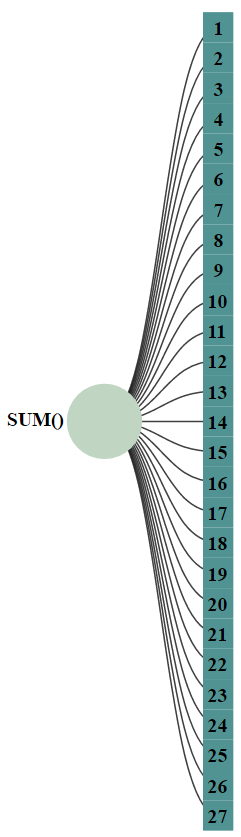
\includegraphics{SUM}
		\label{"fig:sum"} \end{wrapfigure} The discovery of errors and bad design,
	whether by purpose or accident, produced the more jarring events of the study,
	and as such, most users commented on the tool's ability to locate these
	problems in spreadsheet design. This was often supported by the distinctive
	visual signatures of certain bad practices: multiple arguments produce towers
	of nodes, deep function nesting stretches the tree horizontally, and so on. As
	such, the participants remarked on the problems quickly after opening: P3,
	exploring the example for a 27-argument SUM (with SUM's initial appearance
	pictured left), diagnosed the situation with either incompetency or just plain
	weirdness; P2, meanwhile, decided that the spreadsheet's author "was having a
	bad day" when writing an AVERAGE with 18 distinct arguments. Aside from these
	implicit cues, there are also nodes which refer to formula errors, prefixed
	with \#s, which P4 said could be useful if marked well. Furthermore, once these
	errors are found, the participants could then open the offending spreadsheets,
	discovering that, even in context, some of these formulas remained
	incomprehensible, posing problems for mere functioning and maintainability.
	[Hermanns discussed in one of her paper the transfer scenarios -- would go well
	here.] The tool, then, aggregates these issues in a single place, accessible to
	either the unguided user and the ones who know exactly where to find these
	issues. \par The detection of bad design, however, is certainly not limited to
	a visualization tool, and some users remarked that a tool which printed a list
	of errors could suffice just as well for that purpose. However, they also
	remarked that this visual interface better supports the case when searching for
	new and unknown brands of bad smell.
	
	Because the exploratory design makes no qualitative judgment and visualizes
	benign designs with the problematic, it therefore allows for flexible
	interpretation of what is an issue; that is, a user might not realize a certain
	design is suboptimal until they see it in the tree and, at the point, find
	every instance of it.
	
	\subsection{Negative Responses} Some interaction with the tool underlined how a
	lack of contextual information may limit the tool. For example, the benefits
	described in the previous sections imply a hidden complication: if the tool
	educates through example but doesn't explicitly distinguish between good design
	and bad design, how can we be sure that people won't inadvertently learn bad
	design from it. Right now, we can't be sure; the tool would have to be
	
	supplemented with a distinguishing eye, informed on bad design already, and
	supplying the tool with this would take it beyond a design-agnostic view. [More
	on this in the conclusion.] \par Furthermore, just because a user can
	exhaustively explore every variation of how a function was used doesn't mean
	they will learn exactly what it does. P1, in their exploration, examined
	functions that they hadn't used before, such as KURT and PV, and described
	precisely what types of arguments it accepted and how many. However, even after
	exploring the spreadsheets, they could not accurately describe what the
	functions produced without consulting the official documentation. Whether
	through reticence of the tool or obscurity of the functions themselves, the
	exploratory environment is not enough for independent education. However,
	unlike the previous problem, this can be addressed, perhaps, by guiding the
	user directly to such documentation from within the tool without violating any
	design concerns. \par A threat to the exploratory philosophy may also mount
	from the problem of too much data, particularly in the popular functions, like
	SUM and IF. We had added some precautions before the study: for any position in
	the tree, for example, only the ten most common functions were displayed
	without clicking on the expansion arrow 
\includegraphics[scale=.35]{arrow}.
	Nevertheless, P3 remarked that they specifically avoided the most popular
	functions, anticipating a flood of nodes from which they could salvage nothing
	interesting -- which might not have been a bad prediction, considering that the
	SUM is built from 910 nodes and IF, at least 18000 [double-check these with
	refined data]. P2 corroborated this by explaining how they gravitated toward
	specific examples over the plane of nodes but complicates it further by also
	deeming the tool at its best when it shows either every possibility of an
	side-by-side (for comparison) or nothing on that branch at all, a balance that
	is hard to strike with node-dense trees. \par Throughout the study, it became
	apparent that some of the concepts, particularly optional arguments, were
	easily lost in the representation. To illustrate this, consider the following
	two trees: \par 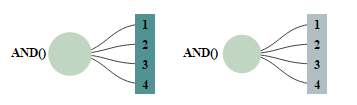
\includegraphics[width = .46\textwidth]{comparison} The
	difference is, perhaps, too subtle: on the left, the tree contains instances of
	AND functions with any number of arguments, up to four; on the right, the tree
	contains only instances with exactly four arguments. In other words, an
	instance of "=AND(A1, B2, C3, D4)" would be found in both trees, while
	"=AND(A1, B2)" would be found in only the left. Though the users naturally did
	not explicitly report misinterpreting the icons, it became clear in their
	out-loud thoughts that they viewed each box as a fundamentally different set of
	possibilities in formula construction rather than just a specific parameter.
	Though we clarified the meanings when these misunderstandings became apparent,
	these events point to a failure in the tool to properly indicate every function
	with clarity.   \par
	
	
	
	\section{Limitations} Beyond the negative responses in the user study, a few
	more inherent limitations beset the tool. These largely resulted from
	trade-offs in which we found no acceptable way to win the best of both worlds,
	and necessary compromises were made. \par Because the data collection depends
	on POI's formula parser, it affords no leeway or partial information from a
	formula; it either processes it perfectly or throws it out. As such, the
	visualization inhibits insight into anything with syntactical errors or
	third-party functions that can't be evaluated without additional tools. Note,
	however, that this does not include standard Excel errors like \#REF! and
	\#DIV/0, which the parser handles well. This poses more egregious problems,
	however, when POI does not support the parsing of certain functions, such as
	EOMONTH (as obscure as it may be), preventing the healthy growth of those
	trees. \par Many functions have an expected order of arguments, but some, like
	SUM and MATCH, can be reordered in various ways and maintain their value.
	However, the representation that this tool uses reinforces for all functions
	that the order is important, even in these exceptions. Future work could design
	a new family of tree to accommodate these loose cases, however, by bucketing
	order-insignificant arguments together; this, of course, would still have to
	address the profusion of co-presented data. \par A larger and related problem
	is the loss of argument combination. In the example in section B, we saw how
	the tools conveys which arguments are used most often on each side of an equals
	sign, but it does not encode how these whether references were actually
	compared to strings and numbers the most or whether it corresponded more to all
	the arguments beneath those two
	
	\section{Conclusion} Why design agnostic?
	
	[to be filled in]
	
	-extensible to other spreadsheets? % conference papers do not normally have an
	% appendix
	
	
	% use section* for acknowledgment
	\section*{Acknowledgment} This material is based upon work supported in whole
	or in part with funding from the Laboratory for Analytic Sciences (LAS). Any
	opinions, findings, conclusions, or recommendations expressed in this material
	are those of the author(s) and do not necessarily reflect the views of the LAS
	and/or any agency or entity of the United States Government.
	
	% references section
	
	% can use a bibliography generated by BibTeX as a .bbl file
	% BibTeX documentation can be easily obtained at:
	% http://mirror.ctan.org/biblio/bibtex/contrib/doc/
	% The IEEEtran BibTeX style support page is at:
	% http://www.michaelshell.org/tex/ieeetran/bibtex/
	\bibliographystyle{IEEEtran} % argument is your BibTeX string definitions and
	% bibliography database(s)
	\bibliography{paper} %
	% <OR> manually copy in the resultant .bbl file
	% set second argument of \begin to the number of references
	% (used to reserve space for the reference number labels box)
	%\begin{thebibliography}{1}
	%
	%\bibitem{IEEEhowto:kopka}
	%H.~Kopka and P.~W. Daly, \emph{A Guide to \LaTeX}, 3rd~ed.\hskip 1em plus
	%  0.5em minus 0.4em\relax Harlow, England: Addison-Wesley, 1999.
	%
	%
	%\end{thebibliography}
	
	
	
	
	% that's all folks
\end{document}


